\documentclass[UTF8]{ctexart}
\CTEXsetup[format={\Large\bfseries}]{section}
\usepackage{geometry}
\usepackage{graphicx}
\usepackage{tcolorbox}
\usepackage{listings}
%\usepackage[usenames,dvipsnames]{xcolor}


\geometry{a4paper,scale=0.8}


\definecolor{mygreen}{rgb}{0,0.6,0}
\definecolor{mygray}{rgb}{0.5,0.5,0.5}
\definecolor{mymauve}{rgb}{0.58,0,0.82}
\lstset{
	backgroundcolor=\color{lightgray}, 
	basicstyle = \footnotesize,       
	breakatwhitespace = false,        
	breaklines = true,                 
	captionpos = b,                    
	commentstyle = \color{mygreen}\bfseries,
	extendedchars = false,             
	frame =shadowbox, 
	framerule=0.5pt,
	keepspaces=true,
	keywordstyle=\color{blue}\bfseries, % keyword style
	language = C++,                     % the language of code
	otherkeywords={string}, 
	numbers=left, 
	numbersep=5pt,
	numberstyle=\tiny\color{mygray},
	rulecolor=\color{black},         
	showspaces=false,  
	showstringspaces=false, 
	showtabs=false,    
	stepnumber=1,         
	stringstyle=\color{mymauve},        % string literal style
	tabsize=2,          
	title=\lstname                      
}


\title{C++作为语言的基础部分学习}
\author{Jiangsu Du}
\date{\today}
	
\begin{document}
\maketitle
学习的教材为《C++ Primer(第五版)》
\tableofcontents


\section{introduction}

如图~\ref{fig:overview},以C++为基本,对基础部分进行学习。
了解C++基本语法,学习类与数据对象,容器和算法,\textbf{面向对象和泛型编程(重点)},编译与底层,C++新特性。

\begin{figure}[]
	\centering
	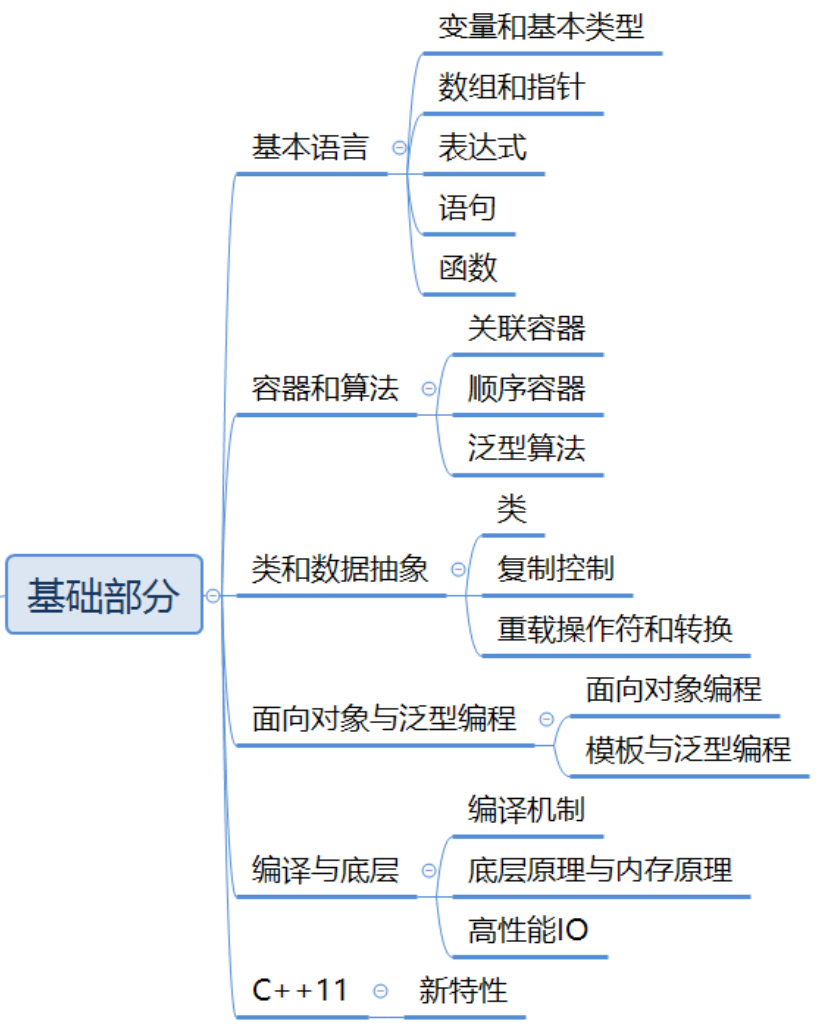
\includegraphics[width=0.5\columnwidth]{pic/overview.png}
	\caption{基础部分学习总览}
	\label{fig:overview}
	% \vspace{-5pt}
\end{figure}

\section{基本语言知识点}
C++语言同时支持四种编程风格:C风格、基于对象、面向对象和泛型。
在C++11之前抽象存在若干的缺陷,最严重的是缺少自动内存管理和对象级别的消息发送机制。

\begin{itemize}
	\item \underline{static}关键字:在全局变量前面的时候,定义一个全局静态变量,在静态存储区,整个程序运行期间一直存在,未被初始化的全局静态变量将自动初始化为0,作用域在声明他的文件之外不可见。相对应的,局部静态变量,大体与全局静态变量是一样的,只是作用域只停留在局部,当方法退出时,全局静态变量不销毁而是继续驻留在静态存储区,直到方法被再次调用。
	\item 
\end{itemize}

\section{一些问题}
\begin{itemize}
\item \textbf{static}关键字:在全局变量前面的时候,定义一个全局静态变量,在静态存储区,整个程序运行期间一直存在,未被初始化的全局静态变量将自动初始化为0,作用域在声明他的文件之外不可见。相对应的,局部静态变量,大体与全局静态变量是一样的,只是作用域只停留在局部,当方法退出时,全局静态变量不销毁而是继续驻留在静态存储区,直到方法被再次调用。
\end{itemize}


\end{document}
